
        \documentclass[tikz]{standalone}
        \begin{document}
        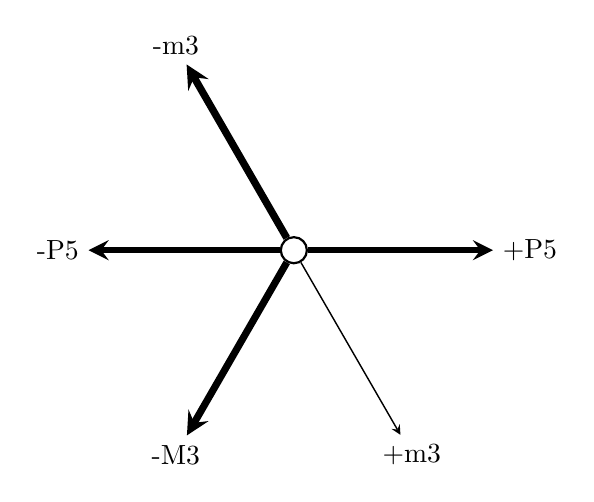
\begin{tikzpicture}[scale=3.5, ->, >=stealth]

        % the circle
        \node (origin) at (0,0) [draw,circle,black,fill=white,thick]{};
        % constant scaling for widths
        \def\cons{10}
        
                \node (0) at +(0*360/6:0.8563709247480386) {+P5};
                \path (origin) edge [line width=\cons*0.21260507528342035] node {} (0);
                
                \node (1) at +(-1*360/6:0.8563709247480386) {+m3};
                \path (origin) edge [line width=\cons*0.05154400246991714] node {} (1);
                
                \node (2) at +(-2*360/6:0.8563709247480386) {-M3};
                \path (origin) edge [line width=\cons*0.25749441353187075] node {} (2);
                
                \node (3) at +(-3*360/6:0.8563709247480386) {-P5};
                \path (origin) edge [line width=\cons*0.21323978433112492] node {} (3);
                
                \node (4) at +(-4*360/6:0.8563709247480386) {-m3};
                \path (origin) edge [line width=\cons*0.2651167243836666] node {} (4);
                
        \end{tikzpicture}
        \end{document}
        